\chapter{Fault-Tolerant computation}
\section{Introduction to fault tolerant computation}
So far we had a sort of communication scenario where Alice wants to send information to Bob and the error occurs in the noisy channel. 
Then we developed good algorithms to contrast errors that happen in between, protecting the information.
To do that we supposed that Alice and Bob were dealing with perfect quantum computers with perfect gates and perfect operations. 
However, nature is far from this. 
The error can occur while we are doing any quantum operations, also during the quantum error correction procedure.
Noise afflicts each of the elements used to build this circuit : the state preparation procedures, quantum logic gates, measurement of the output, and even the simple transmission of quantum information along quantum wires.

To face this problem we can use fault-tolerant computation, which computes directly on encoded quantum states in such a manner that decoding is never required. Hence, each qubit in the original circuit is replaced with an encoded block of qubits, using an error-correcting code such as the seven qubit Steane code, and each gate in the original circuit is replaced with a procedure for performing an encoded gate acting on the encoded state. 
One might think performing error-correction periodically after every operation, but this is not sufficient to prevent the build-up of errors.
%Two are the reasons: first, the encoded gates can cause errors to propagate and second is that error-correction itself can introduce errors on the encoded qubits, so we must be careful to design error-correction procedures that do not introduce too many errors into the encoded data
%%%%%%%%%
%Aggiusta 
%%%%%%%%%%
% In fact, one of the most powerful applications of quantum error-correction is not merely the protection of stored or transmitted quantum information, but the protection of quantum information as it dynamically undergoes computation.
% Moreover, a fault-tolerant computation and protocols prevent from catastrophic events of error propagation by ensuring that a single faulty gate or time step produces only a single error in each block of quantum error correction codes. Hence, a fault tolerant computation is that the circuits used for gate operations and error correction procedures should not cause errors to cascade or propagate along the circuit.
%%%%%%%%%
%ERROR PROPAGATION
%%%%%%%%%

In fact, when we perform multiple qubits gates during a quantum computation, any existing error can propagate to other qubits, even if the gate itself can be considered perfect.
For instance, a CNOT gate can propagate forward (from control qubit to the target qubit) a bit-flip error. In figure \ref{fig:CNOT_prop} a bit-flip error occurs on the control qubit just before the CNOT gate.
This single error will cascade forward (from control to target) such that the X error propagates on both output qubits after the gate.

We started with 1 error and we ended up with 2 errors. 
\begin{figure}[h!]
    \centering
    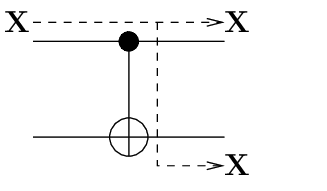
\includegraphics[scale=0.5]{Mainmatter/images/XCNOT.png}
    \caption{A CNOT gate can cause a X error to propagate forward so that instead of affecting one qubit, it affects two. This is also true when encoded qubits are used, and an encoded CNOT is implemented.}
    \label{fig:CNOT_prop}
\end{figure}

Another example, that has not any classical analogy, is the backwards (from target to control) propagation. Imagine having a CNOT and a Z error occurs just before on the target qubit, then after the CNOT we will have 2 phase errors on both qubits as shown in figure \ref{fig:CNOT_prop2} .

\begin{figure}[h!]
    \centering
    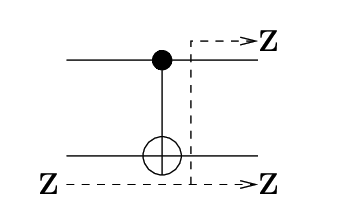
\includegraphics[scale=0.5]{Mainmatter/images/ZCNOT.png}
    \caption{A CNOT gate can cause a Z error to propagate backwards so that instead of affecting one qubit, it affects two. This is also true when encoded qubits are used, and an encoded CNOT is implemented.}
    \label{fig:CNOT_prop2}
\end{figure}
This is clearly a problem if we build an arbitrary circuit that implements CNOT gates and a QECC that corrects up to 1 error, it is not able to correct the propagated error anymore.
Thus, by error propagation, a correctable local error is converted into a non-correctable one. The procedure described is thus not fault tolerant.




Hence, to achieve a fault tolerant computation we first need to implement fault tolerant logic operations, which prevent the building up of errors in the same error correction block. A solution is to perform logic gates transversally - i.e. a transversal gate interacts the ith qubit in one block with the ith qubit of the other block. Recall single encoded qubit gates involving only one block are transversal, because the ith qubit interacts with itself.
For instance, in the Steane code the logical $\Bar{X}=X^{\otimes 7} $ and $\Bar{Z}=Z^{\otimes 7}$ operations on a single encoded
qubit are the first examples of valid transversal codeword operations.
% The spreading of single-qubit errors during imperfect gates to more than one qubit in the output can be prevented if the gates are implemented in a transversal manner. That is, the gates shall be implemented using only independent operations on each of the physical qubits. Logical gates that are implemented in this way are naturally fault-tolerant since any error on a single physical qubit can not propagate to another physical qubit in the encoded state.
For any stabilizer codes, a large class of operations can be performed on logical data in a fault-tolerant way. 
Furthermore, the performed operations must map codewords to codewords.



More precisely, if a given logical state, $|\psi\rangle_{L}$ is stabilized by $M \in \mathcal{S}$, and the logical operation $U$ is applied, the new state, $U|\psi\rangle_{L}$ is stabilized by $U M U^{\dagger} \in \mathcal{S}$, i.e,
\begin{equation}
(U M U^{\dagger}) U|\psi\rangle_{L}=U M|\psi\rangle_{L}=U|\psi\rangle_{L}
\end{equation}
Hence, for $U$ to preserve the codespace, $U M U^{\dagger}$ must be in the stabiliser set.
This properties is satisfied for any $U \in \mathbf{C}$ where $\mathbf{C}$ is called the Clifford group:
\begin{definition}
Let $\mathcal{P}_{n}$ be the Pauli group on $n$ qubits and let $\mathcal{U}\left(2^{n}\right)$ be the unitary group. The Clifford group $\mathbf{C}_{n}$ on $n$ qubits is,
\begin{equation}
\mathbf{C}_{n}=\left\{U \in \mathcal{U}\left(2^{n}\right): U P U^{\dagger} \in \mathcal{P}_{n} \text { for all } P \in \mathcal{P}_{n}\right\}
\end{equation}
The Clifford group on $n$ qubits can be generated by Hadamard gate $H, R_{\pi / 4}$ gate, and CNOT gate, where
$$
H=\frac{1}{2}\left(\begin{array}{cc}
1 & 1 \\
1 & -1
\end{array}\right), \quad R_{\pi / 4}=e^{-i \pi / 4}\left(\begin{array}{cc}
1 & 0 \\
0 & i
\end{array}\right), \quad \operatorname{CNOT}=\left(\begin{array}{cccc}
1 & 0 & 0 & 0 \\
0 & 1 & 0 & 0 \\
0 & 0 & 0 & 1 \\
0 & 0 & 1 & 0
\end{array}\right) .
$$
\end{definition}
From this we can notice also how error how errors change after applying quantum gates: 
the operation of $U$ on an erroneous codeword $E|\psi\rangle$ gives,
\begin{equation}
U E|\psi\rangle=\left(U E U^{\dagger}\right) U|\psi\rangle
\label{eq:spread}
\end{equation}
Observe that $U|\psi\rangle$ is a state from the operation of $U$ on state $|\psi\rangle$.
Here we can see that the error $E$ before the operation $U$ becomes $U E U^{\dagger}$ after the operation of $U$. 
So now our goal is to implement the generators of clifford group in a fault-tolerant way. Let us think this in the context of the seven qubit code $[[7,1,3]]$ with its stabiliser set (\ref{eq:stabSteane}). 

\subsection*{Fault-tolerant Hadamard and $R_{\pi/4}$}
A logical Hadamard gate $\bar{H}$ interchanges $\bar{Z}$ and $\bar{X}$ under conjugation, just as the Hadamard gate $H$ interchanges $Z$ and $X$ under conjugation. $\bar{H}= H^{\otimes 7}$ accomplishes this task, so that a Hadamard on the encoded qubit can be implemented as in figure \ref{fig:logHada}
\begin{figure}[h!]
    \centering
    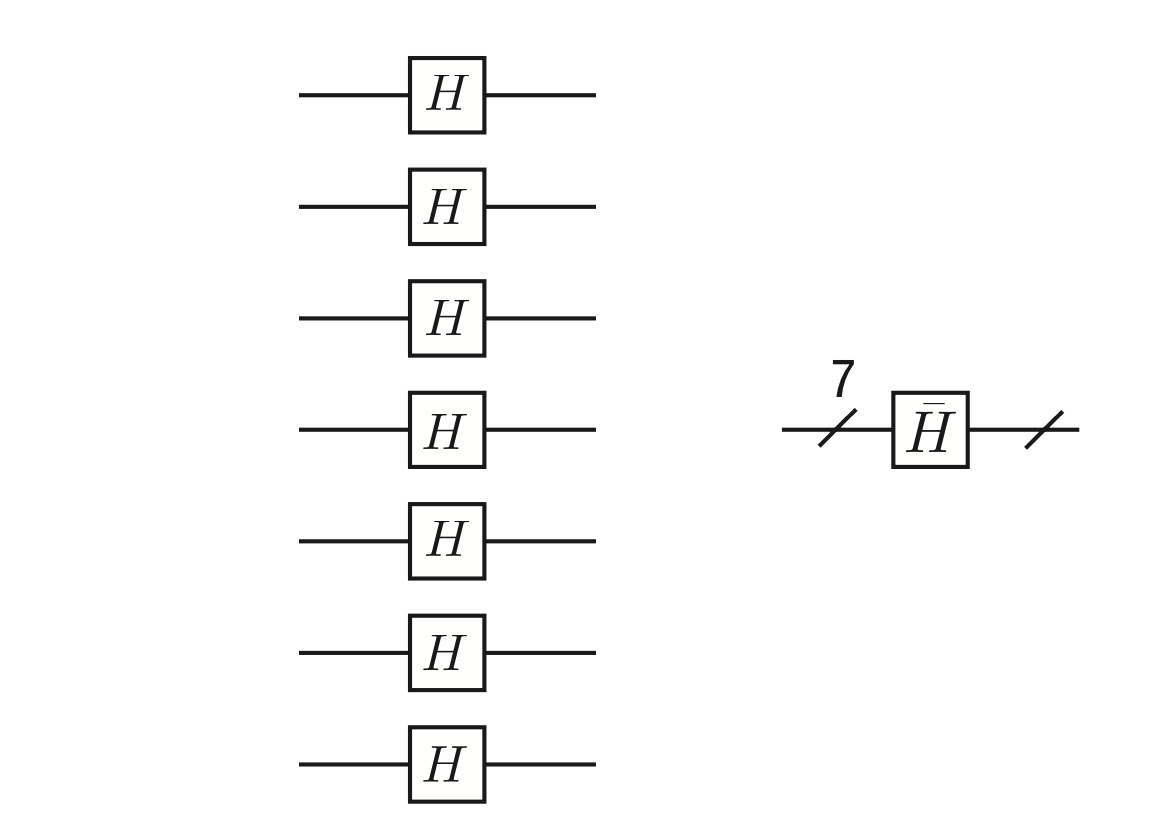
\includegraphics[scale=0.5]{Mainmatter/images/LogicalHadamard.png}
    \caption{This figure shows the logical hadamard gate. On the right is showed a more compact notation, the 7 and the slash on the wire indicate that we are operating on an encoded state}
    \label{fig:logHada}
\end{figure}

This is fautl-tolerant because the failure of a single component in the circuit can cause at most one error in the block of qubits output from the procedure. To see that this is true suppose that a $Z$ error occurs on the first qubit just before the encoded $H$ gate was applied. The combined operation on the qubit is $H Z$. Then, we can use the equation \ref{eq:spread}, which describes how an error spreads after applying a gate, hence it gives $H Z =(H Z H^{\dagger})H=X H$, so such an error is equivalent to first applying $H$ then the error $X$ occurring.

Moreover, $\Bar{H}$ maps stabilisers in other stabiliser, let us take the first stabilizer $M_1=ZZZZIII \in \mathcal{S}$ and we see that $\Bar{H} M_1 \Bar{H} = M_4 =XXXXIII $ which is still in the stabilizer. 

A very similar construction can be implemented also for the $\frac{\pi}{4}$ logical operation.  The $\frac{\pi}{4}$ rotation gate single qubit $R_{\pi/4}$ gate leaves $Z$ unaltered, while $X$ is mapped to $Y=iXZ$. However, applying 
$\Bar{R_{\pi/4}}=R_{\pi/4}^{\otimes7}$ takes $\bar{Z}$ to $\bar{Z}$ under conjugation, and $\bar{X}$ to $-\bar{Y}.$ The minus sign in front of the $-\bar{Y}$ may be fixed up by applying $\bar{Z}$.
Thus, applying the operation $Z R_{\pi/4}$ to each qubit in the code effects an encoded phase gate, which is transversal and thus fault-tolerant.


\subsection*{Fault-tolerant CNOT gate}

A two qubit logical CNOT operation can also be applied in the same transversal way. For un-encoded qubits, a CNOT operation performs the following mapping on the two qubit stabilizer set,
$$
\begin{array}{l}
X \otimes I \rightarrow X \otimes X \\
I \otimes Z \rightarrow Z \otimes Z \\
Z \otimes I \rightarrow Z \otimes I \\
I \otimes X \rightarrow I \otimes X .
\end{array}
$$
Where the first operator corresponds to the control qubit and the second operator corresponds to the target. This can be extended to the logical space, we can apply the logical CNOT operation between two encoded states: 
$$
\begin{array}{l}
\bar{X} \otimes I \rightarrow \bar{X} \otimes \bar{X}, \\
I \otimes \bar{Z} \rightarrow \bar{Z} \otimes \bar{Z}, \\
\bar{Z} \otimes I \rightarrow \bar{Z} \otimes I, \\
I \otimes \bar{X} \rightarrow I \otimes \bar{X} .
\end{array}
$$
The issue of Fault-tolerance with these logical operations should be clear. The $\bar{X}, \bar{Z}, \bar{H}$ and $\bar{R}_{\frac{\pi}{4}}$ gates are fault-tolerant since the logical operation is performed through seven single qubit gates. The logical CNOT is also fault-tolerant since each two-qubit gate only operates between counterpart qubits in each logical block as shown in figure \ref{fig:TransCNOT} . Hence if any gate is inaccurate, then at most a single error will be introduced in each block, and we are able to correct 1 error per block. 
\begin{figure}[h!]
    \centering
    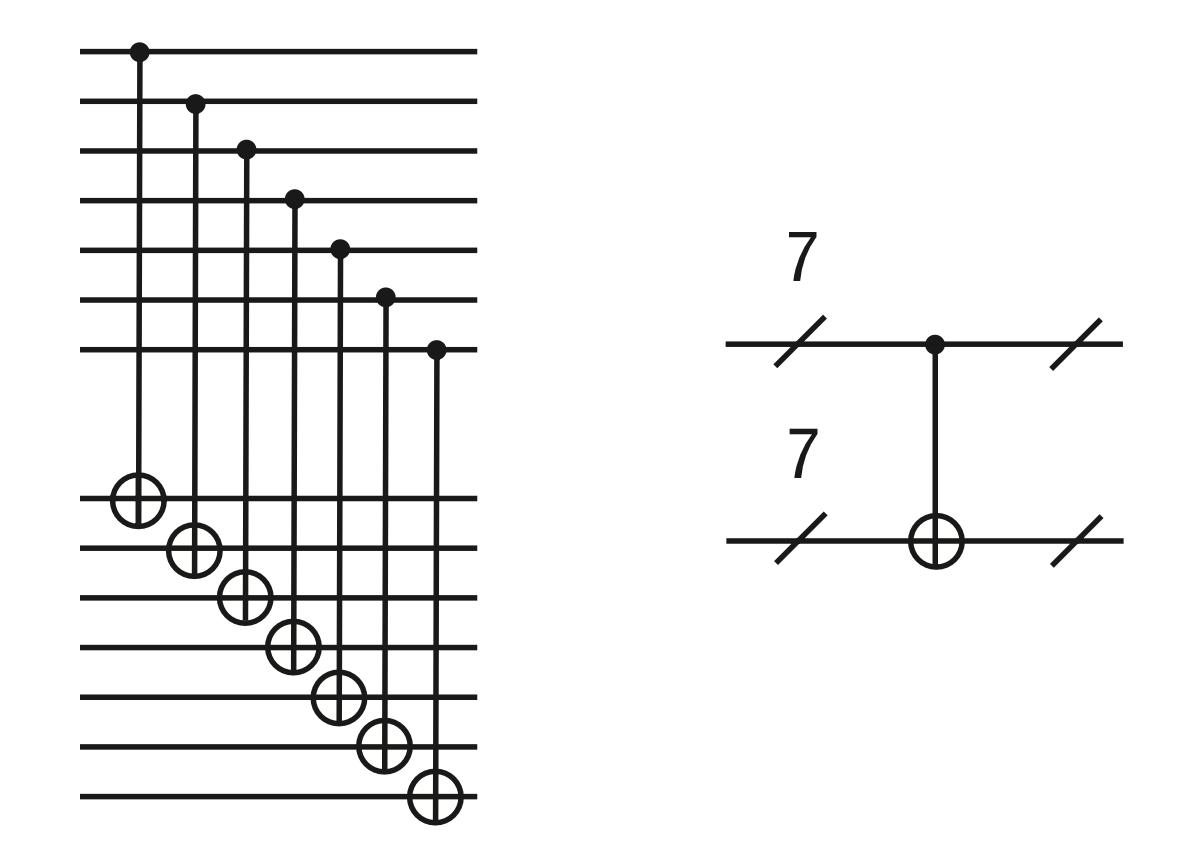
\includegraphics[scale=0.5]{Mainmatter/images/Transversal_CNOT.png}
    \caption{This figure shows a transversal fault-tolerant CNOT between two encoded qubits.}
    \label{fig:TransCNOT}
\end{figure}
A fault-tolerant CNOT is also a good example to show that the error probability goes from $p$ to $cp^2$.
%Might add that probability of 1 error goes from p to p^2
% In contrast to the $[[7,1,3]]$ code, let us also take a quick look at the $[[5,1,3]]$ code. The $[[5,1,3]]$ code is a non-CSS code, the Clifford group of gates cannot be fully implemented in transversal manner. To see this clearly we can examine how the stabilizer group for the code transforms under transversal Hadamard operation:
% $$
% \left(\begin{array}{ccccc}
% X & Z & Z & X & I \\
% I & X & Z & Z & X \\
% X & I & X & Z & Z \\
% Z & X & I & X & Z
% \end{array}\right) \quad \longrightarrow\left(\begin{array}{ccccc}
% Z & X & X & Z & I \\
% I & Z & X & X & Z \\
% Z & I & Z & X & X \\
% X & Z & I & Z & X
% \end{array}\right)
% $$
% The stabilizer group is not preserved under this transformation, therefore the transversal Hadamard operation is not valid for the $[[5,1,3]]$ code. One thing to briefly note that there is a method for performing logical Hadamar and phase gates on the $[[5,1,3]]$.

Nevertheless, the Clifford group is not an universal set of operation.  
The Gottesman-Knill theorem states that if a quantum circuit consists of only these elementary operations, the operation of the circuit can be efficiently simulated by a classical computer \cite{gottesman1998heisenberg}. This means that if we want to construct a quantum computer that fully exploits the power of quantum computation, only aforementioned operations are not sufficient.

In order to achieve universality one of the following gates are generally added to the available set: $R_{\pi/8}$ or the Toffoli gate. 
Although both gates can be implemented in a fault-tolerant way through a more complicate procedure called "Magic state injection", in the following it will focus only the fault-tolerant implementation of  $R_{\pi/8}$ gate. 

The basic idea of this procedure is based on the concept of teleportation, which is briefly described in the appendix.
Let us begin by not worrying about fault-tolerance, and simply attempt to perform some gate $\bar{U}$ on an encoded state. 
We will consider the case of a single-qubit gate $\Bar{U}$ first. \cite{gottesman2009introduction}

\begin{figure}[h!]
    \centering
    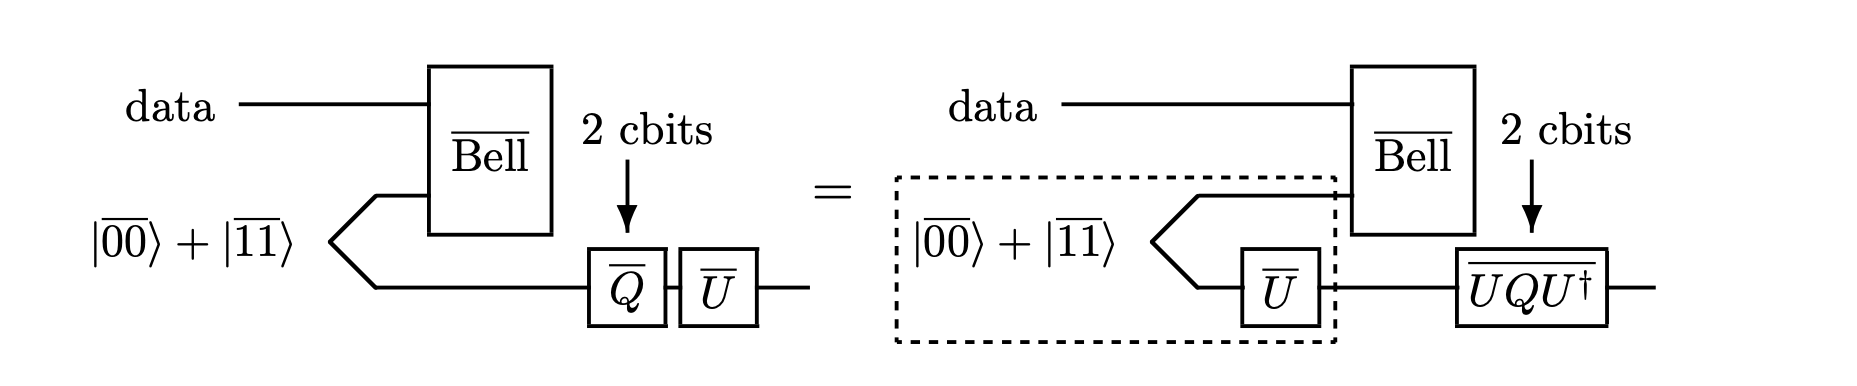
\includegraphics[width=\textwidth]{Mainmatter/images/teleportation_fault.png}
    \caption{Gate teleportation of $\Bar{U}$. The process of teleporting the state followed by $\Bar{U}$ is the same as teleporting the state through a special ancilla with an appropriately modified correction operation.}
    \label{fig:fault_teleport}
\end{figure}
Suppose we were to perform quantum teleportation (this means to apply the require pauli $\Bar{Q}$ gates once we get the instructions from classical measurements) and then follow it, somehow, by an implementation of $\Bar{U}$. Thus on input state $\ket{\psi}$, the overall output state would be $U\ket{\psi}$. 
Now imagine that the receiver (Bob), who controls the output block, perform $\Bar{U}$ earlier than intended, before the senders’s (Alice) measurement outcome instructions.
Eventually Alice performs the logical Bell measurement and sends Bob the two classical bits describing the outcome, corresponding to a logical Pauli $\Bar{Q}$.
To complete the teleportation procedure, Bob needs to do something different now, he can't do the same pauli operation as before: first, he must undo the $\bar{U}$ he performed prematurely, then perform $\Bar{Q}$, and then finally redo $\bar{U}$, now in the correct place. That is, he should implement the gate $\Bar{U}Q\Bar{U}^{\dagger}$. This procedure is pictured in figure $\ref{fig:fault_teleport}$. It may not seem like we have gained anything by doing this, but for some special gates $U$, we have. We can imagine the state $(I \otimes \bar{U})(|\overline{00}\rangle+|\overline{11}\rangle)$ as a special ancilla state, a replacement for the EPR pair normally used in teleportation, and we can prepare it separately. Since it is a fixed ancilla state, independent of the data, we can apply some special tricks to preparing it.

We still have to perform the gate $\Bar{U} \Bar{Q}\Bar{U^{\dagger}}$, which cannot be done ahead of time on the ancilla, since $Q$ depends on the outcome of a logical Bell measurement on the data block. However, the gate $\Bar{U} \Bar{Q}\Bar{U^{\dagger}}$ might be simpler to perform than $\bar{U}$ was. For instance, when $U \in \mathbf{C}_{1}, \bar{U} \bar{Q} \bar{U}^{\dagger} \in \mathcal{P}_{1}$ that is the defining property of the Clifford group. For some gates $U \notin \mathcal{C}_{1}$, it is nonetheless still true that $\bar{U} \bar{Q} \bar{U}^{\dagger} \in \mathbf{C}_{1}$ for any $\bar{Q} \in \mathcal{P}_{1}$. For instance, the $\pi/8$ rotation $R_{\pi/8}$ has this property:
$$
\begin{array}{l}
R_{\pi / 8} X R_{\pi / 8}^{\dagger}=\left(\begin{array}{cc}
0 & e^{-i \pi / 4} \\
e^{i \pi / 4} & 0
\end{array}\right)=e^{i \pi / 4} X P^{\dagger} \\
R_{\pi / 8} Z R_{\pi / 8}^{\dagger}=Z
\end{array}
$$
We sometimes call the set of unitary operators with this property, of conjugating Pauli operators into Clifford group operators, $C_{3} . C_{1}$ is the Pauli group $\mathcal{P}_{n}$, and $C_{2}$ is the Clifford group $\mathcal{C}_{1} .$
One can define a set $C_{k}=\left\{U \mid U Q U^{\dagger} \in C_{k-1} \forall Q \in C_{1}\right\}$, and the teleportation construction tells us how, given appropriate ancilla states, to perform a gate from $C_{k}$ once we know how to perform gates from $C_{k-1}$.

This whole procedure gives us an indication of how to perform a universal set of fault-tolerant gates. For the 7-qubit code, and some similar CSS codes, we already know how to perform all logical Clifford group operations. The Bell measurement is a Clifford group operation, and now we have seen that $R_{\pi / 8} Q R_{\pi / 8}^{\dagger}$ is also a Clifford group operation for $Q \in \mathcal{P}$.  


The correction required after teleportation is a Clifford group gate, for which we already know a fault-tolerant procedure. This yield to the possibility to have universal quantum computation procedure in a complete fault-tolerant way.





\section{Threshold theorem}



The threshold theorem is one of the most remarkable results in fault-tolerant computation. It says that if the error rate of a physical system is below some threshold value, arbitrarily long reliable fault-tolerant quantum computation is possible.




One possible way to prove the threshold theorem and build a reliable quantum computation is by using fault tolerant protocols and concatenating codes.
If an error occurs during a logical gate operation, then Fault-tolerance ensures this error will only propagate to at most one error in each encoded block, after which a cycle of error correction will remove the error. Hence if the failure probability of un-encoded qubits per time step is $p$, then a single level of error correction will ensure that the logical step fails only when two (or more) errors occur. Hence the failure rate of each logical operation, to leading order, is now $p_L = cp^2$, where $p_L$ is the failure rate (per logical gate operation) of a first level logical qubit, and $c$ is the upper bound for the number of possible 2-error combinations which can occur at a physical level within the circuit\footnote{In this specific case $c$ is the number of possible 2-error combinations, because we used a QECC that can correct 1 error. If we use different QECC codes that corrects t-errors the upper bound $c$ becomes: $c=\left(\begin{array}{c}
       G\\
       t+1
 \end{array}\right)$ where G is the total number of gates. 
 
 
 In addition, the logical step fails only when $t+1$ (or more) errors occur. Hence, the failure rate of each logical operation gate, to leading order, is $p_k = cp^{(t+1)}$
 
 
 }.
Hence, thanks to fault tolerance protocols we can decrease the error rate from $p \to cp^2$. 
% If an error occurs during a logical gate operation, then fault-tolerance ensures this error will only propagate to at most $t$ correctable error (depending on which QECC we use) in each encoded block, after which a cycle of error correction that correct $t$ errors will remove them. If the failure probability of un-encoded qubits per time step is $p$, then a single concatenation level of error correction will ensure that the logical step fails only when $t+1$ (or more) errors occur. Hence, the failure rate of each logical operation gate, to leading order, is now $p_k = cp^{(t+1)}$.
% $p_k$ is the failure rate (per logical gate operation) of a first level logical qubit, and $c=\left(\begin{array}{c}
%       G\\
%       t+1
% \end{array}\right)$ where G is the total number of gates. This coefficient is the upper bound for the number of possible ($t+1$)-error combinations if we use a $t$-error correction code, which can occur at a physical level within the circuit.


% For the sake of clarity, in the following lines we suppose that we use a QECC that corrects 1 error. 
% Hence, thanks to fault tolerance protocols we can decrease the error rate from $p \to cp^2$. 
Then, we can reduce the effective error rate achieved even more by concatenation of codes. 
This idea replaces each physical qubit at layer $k$ by an encoded qubit. An example of concatenation using the bit-flip code is shown in figure \ref{fig:codeconc} \footnote{Of course the bit-flip code is insufficient in general since it doesn’t correct phase errors. However, everything we shall demonstrate with the bit-flip code also holds for more general quantum codes, as the 7 qubit code.}.
\begin{figure}[h!]
    \centering
    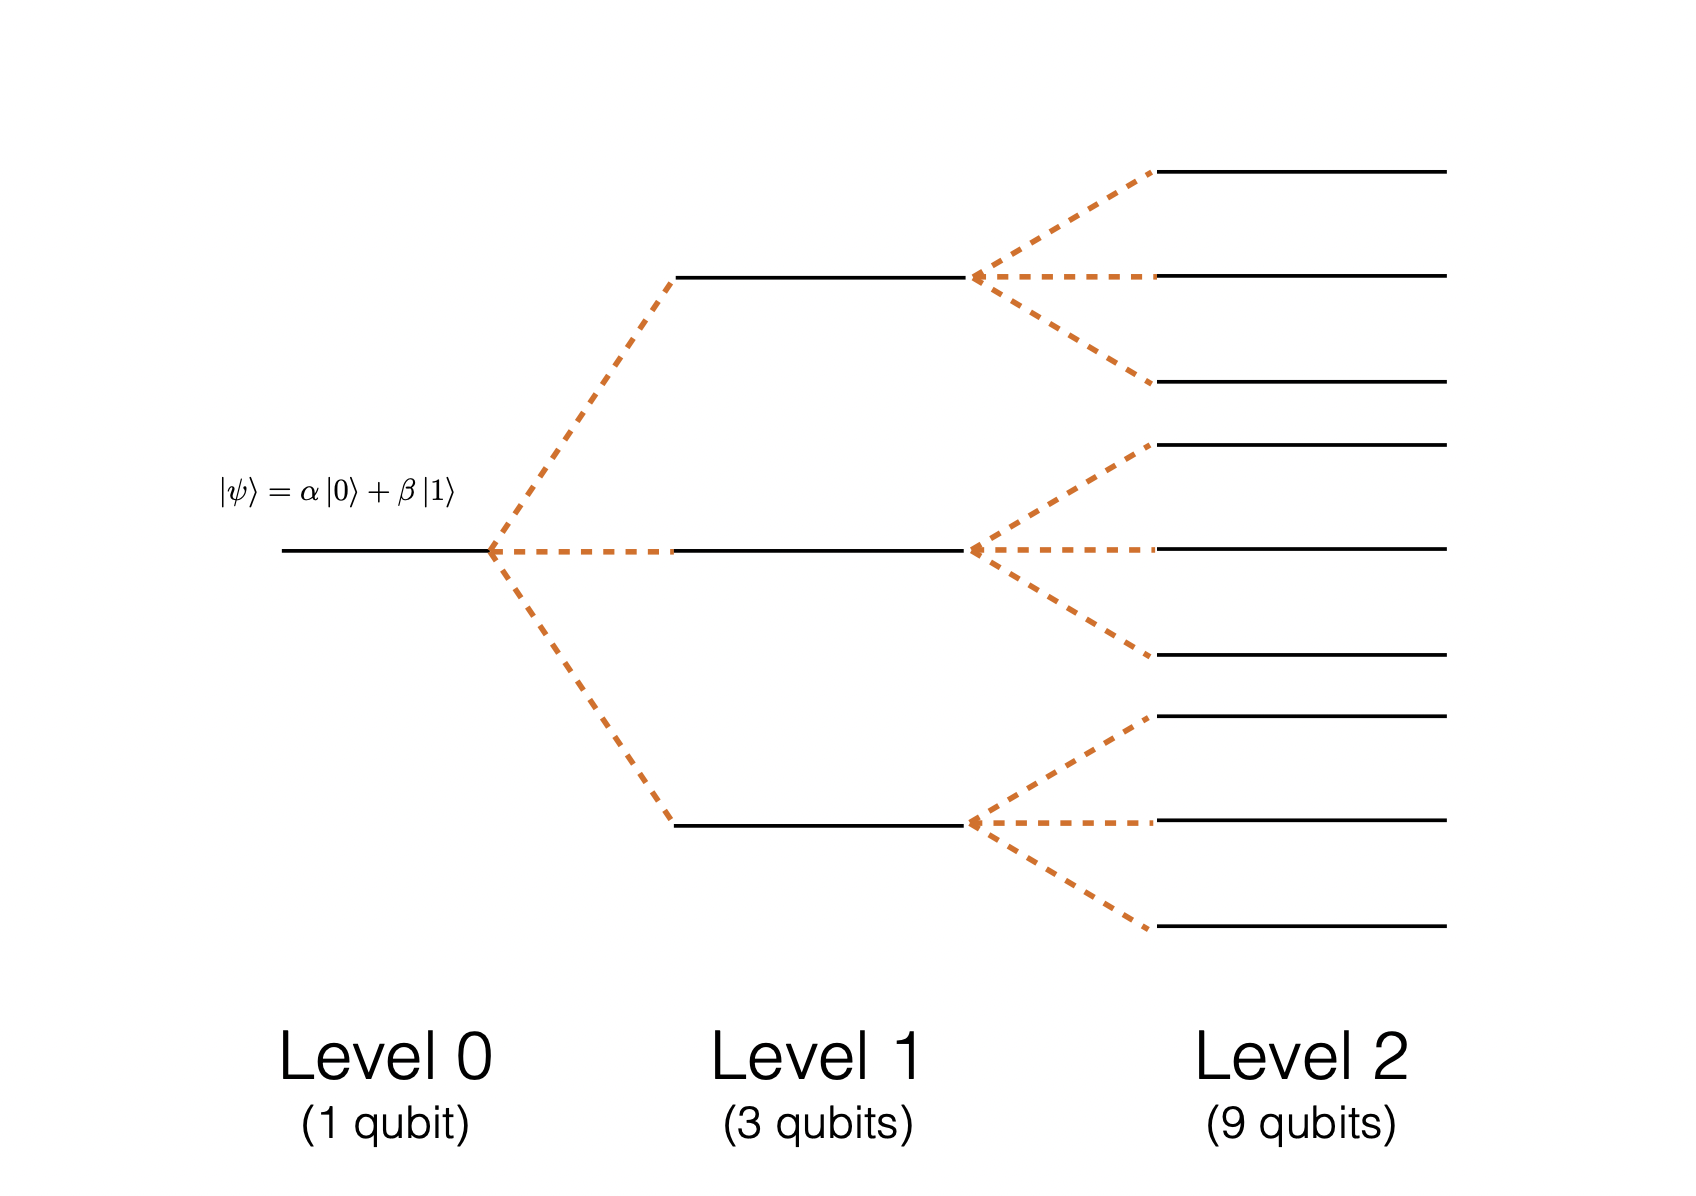
\includegraphics[scale=0.5]{Mainmatter/images/concatenation.png}
    \caption{An illustration of concatenation of the bit flip code. Each qubit at level $k$ is encoded into three qubits at level $k + 1$.}
    \label{fig:codeconc}
\end{figure}

If we perform error correction at each layer of concatenation, then if the bare qubit experiences an error probability of $p$, then after one layer of error correction the logical error probability is $c p^{2}$, and after two layers, the logical error probability is $c\left(c p^{2}\right)^{2}$ (since two blocks have to fail and each block has failure probability $\left.c p^{2}\right)$. With each concatenation later, even though the number of qubits is grows exponentially in k, we get a gain in error probability. That is:
$$
\begin{array}{cccccccccc}
\text { level } 0 & & \text { level } 1 & & \text { level } 2 & & \ldots  & & \text { level } k\\
p &\rightarrow & c p^{2} &\rightarrow & c\left(c p^{2}\right)^{2} &\rightarrow& \ldots &\rightarrow& c^{-1}(c p)^{2^{k}}
\end{array}
$$
And we are guaranteed that this is a gain $(i . e .$, that the error probability decreases with level of concatenation) if
\begin{equation}
p > c p^2
\label{eq:plesscpp}
\end{equation}

Now let us look at the cost of doing this concatenated coding. If the size of the original (unencoded) circuit we want to execute has T gates, and the cost of implementing each gate at the logical level (this depends on the code being used) is at most N physical gates, then the number of gates needed at level 1 of concatenation is at most NT. And for each level of increasing concatenation we must use N times as many gates:
$$
\begin{array}{cccccccccc}
\text { level } 0 & & \text { level } 1 & & \text { level } 2 & & \ldots  & & \text { level } k\\
T &\rightarrow & NT &\rightarrow & N^2T & \rightarrow & \ldots &\rightarrow& N^kT
\end{array}
$$


Note that the number of gates needed grows exponentially in k, but recall that the error probability reduced doubly exponentially in k. This suggests that we can win with this approach. But to see this convincingly, let us see how many gates we need to achieve a given error probability in the computation. Suppose we wish to achieve a final accuracy of $\epsilon \geq 0$ in our simulation of our algorithm.
Then we want that the total error rate is below $\epsilon$: 
$$
T p_{k}=T c^{-1}(c p)^{2^{k}}<\epsilon
$$
for some concatenation level $k$. Here $T$ is the number of logical quantum gates needed to perform the computation (which is the same as the number of gates necessary at the unencoded level), and $p_{k}$ is the error probability per logical gate at concatenation level $k$.


We can solve for $k$ to get
$$
\begin{aligned}
&(c p)^{2^{k}}<\frac{\epsilon c}{T} \\
\Rightarrow \quad & 2^{k}<\log _{c p}\left(\frac{\epsilon c}{T}\right)=\frac{\log_2 \left(\frac{\epsilon c}{T}\right)}{\log_2 (c p)} \\
\Rightarrow \quad & k<\log_2 \left[\frac{\log_2 \left(\frac{\epsilon c}{T}\right)}{\log_2 (c p)}\right]
\end{aligned}
$$
From this upper bound on the concatenation level we can also form an upper bound the number of physical gates we will need to achieve this level $\epsilon$ of logical error. 

We calculated above that at concatenation level $k$ we need $N^{k} T$ gates. Then,
$$
N^{k} T<N^{\log \left(\frac{\log \left(\frac{\epsilon c}{T}\right)}{\log (c p)}\right)} R
$$


But using $\log _{a} x=\frac{\log _{b} x}{\log _{b} a}$, we simplify
$$
N^{\log (\cdot)}=\left(N^{\log _{N}(\cdot)}\right)^{\frac{1}{\log _{N} 2}}=(\cdot)^{\log N}
$$
Using this, the number of gates needed is upper bounded by
$$
\# \text{gates} = T\left(\frac{\log \left(\frac{T}{\epsilon c}\right)}{\log \left(\frac{1}{c p}\right)}\right)^{\log N} \sim  O(T\operatorname{poly}(\log T / \epsilon))
$$
The original $T$ gates are scaled by the factor in braces. This factor is a polynomial in the log (is polylog) in $\frac{1}{\epsilon}$ (inverse error) and in $T$ (the number of gates in the unencoded computation). Therefore the cost of achieving arbitrary error by concatenation scales very favorably, and this is the power of the fault tolerance theorem: we can achieve an arbitrary error probability $\epsilon$ with resources that scale only polylogarithmically in the inverse of the desired error and the complexity of the computation to be performed $(T)$.

Now, let us go back to Eq. \ref{eq:plesscp}, which defines the crucial condition for concatenation to be effective: $p>c p^{2}$. We can compute the value of $p$ that is at the boundary defined by this condition, $p=c p^{2}$. This value of $p$ is called the threshold probability, and is easily seen to be
$$
p_{\mathrm{th}}=c^{-1}
$$
because we want that the error probability decreases further the concatenation goes on.
Thus if the physical error probability is below this threshold probability $p<p_{\mathrm{th}}$, then concatenation and error correction is beneficial. Finally, writing the logical error probability at concatenation level $k$ in terms of $p_{\mathrm{th}}$ gives us
$$
p_{k}=c^{-1}(c p)^{2^{k}}=p_{\mathrm{th}}\left(\frac{p}{p_{\mathrm{th}}}\right)^{2^{k}}
$$

%%%%%%%%%%%
%Da fare
%%%%%%%%%%%
% The behavior of this quantity as a function of $p$, for a fixed $p_{\mathrm{th}}$ and $k$. You will see that if $p$ is a little below the threshold probability the logical error probability quickly goes to zero. In contrast, if $p$ is a little above the threshold probability the logical error probability goes up very quickly. Thus, $p_{\mathrm{th}}$ defines a sharp boundary that specifies when reliable computation is possible and when it is not.


So what is the value of $p_{th}$? This depends heavily on the type of error correction code used, because $c$ depends on the the type of constructions used for gates, measurements, state preparation, etc. Nevertheless, a rough estimate for the threshold probability for the Steane code is given in \cite{Chuang} and the threshold is $p_{th} \approx 10^{-4}$. Thus, if we can get the error rate per gate below this value we can do arbitrary long reliably quantum computation. So if quantum computing architectures can get their fundamental errors (in gates, measurements, state preparation, and idle periods) down to this level, then theory comes in and we are in a safe space to compute.

A more detailed derivation of the threshold theorem can be found in \cite{DanielGottesman}








% This construction can be can be used to reduce the effective error rate achieved by the computation even further. This idea replaces each physical qubit at layer k by an encoded qubit. So the circuit is built by constructing a hierarchy of quantum circuits $C_0$ (the original circuit we wish to simulate), $C1$, $C2$, . . .
% Then if we perform fault tolerant computation and error correction at each layer of concatenation, then if the bare qubit experiences an error probability of $p$, then after one layer of error correction the logical error probability is $cp^2$. In particular if we implement this procedure more and more we decrease the error probability, for example after two layers, the logical error probability is $c(cp^2)^2$ (since two blocks have to fail and each block has failure probability $cp^2$)
% In the first stage of this construction, each qubit in the original circuit is encoded in a quantum code whose qubits are themselves encoded in a quantum code, whose own qubits are encoded yet again, and so forth ad infinitum, as illustrated:
% What is concatenate code? Imagine to encode one qubit with n physical qubits, and then use fault tolerant protocols for gates. If an error occurs in a gate with probability $p$, the probability to have 2 errors goes with the order of $p^2$. By encoding it the effective error rate goes from $p \to Cp^2$, where C is a constant depending on the number of gates that can go wrong. This is an improvement. Concatenate codes make this error falling down smaller and smaller





\section{Toric code}
An active research field in quantum computing is to find codes that will increase $p_{th}$ to larger values. One of the codes that has had a lot of positive feedback and opens up to a larger class of codes (surface codes) is the Toric code.

